%----------------------------------------------------------------------------
%bb defines the bounding box for the pdf
%viewport defines the area of the pdf used
%in sidewaysfigure the last entry in bb moves the caption toward/away the pic
%in sidewaysfigure the second entry in bb moves the pic toward/away the caption
%----------------------------------------------------------------------------
\begin{figure}
\scalebox{0.8}[0.8]{
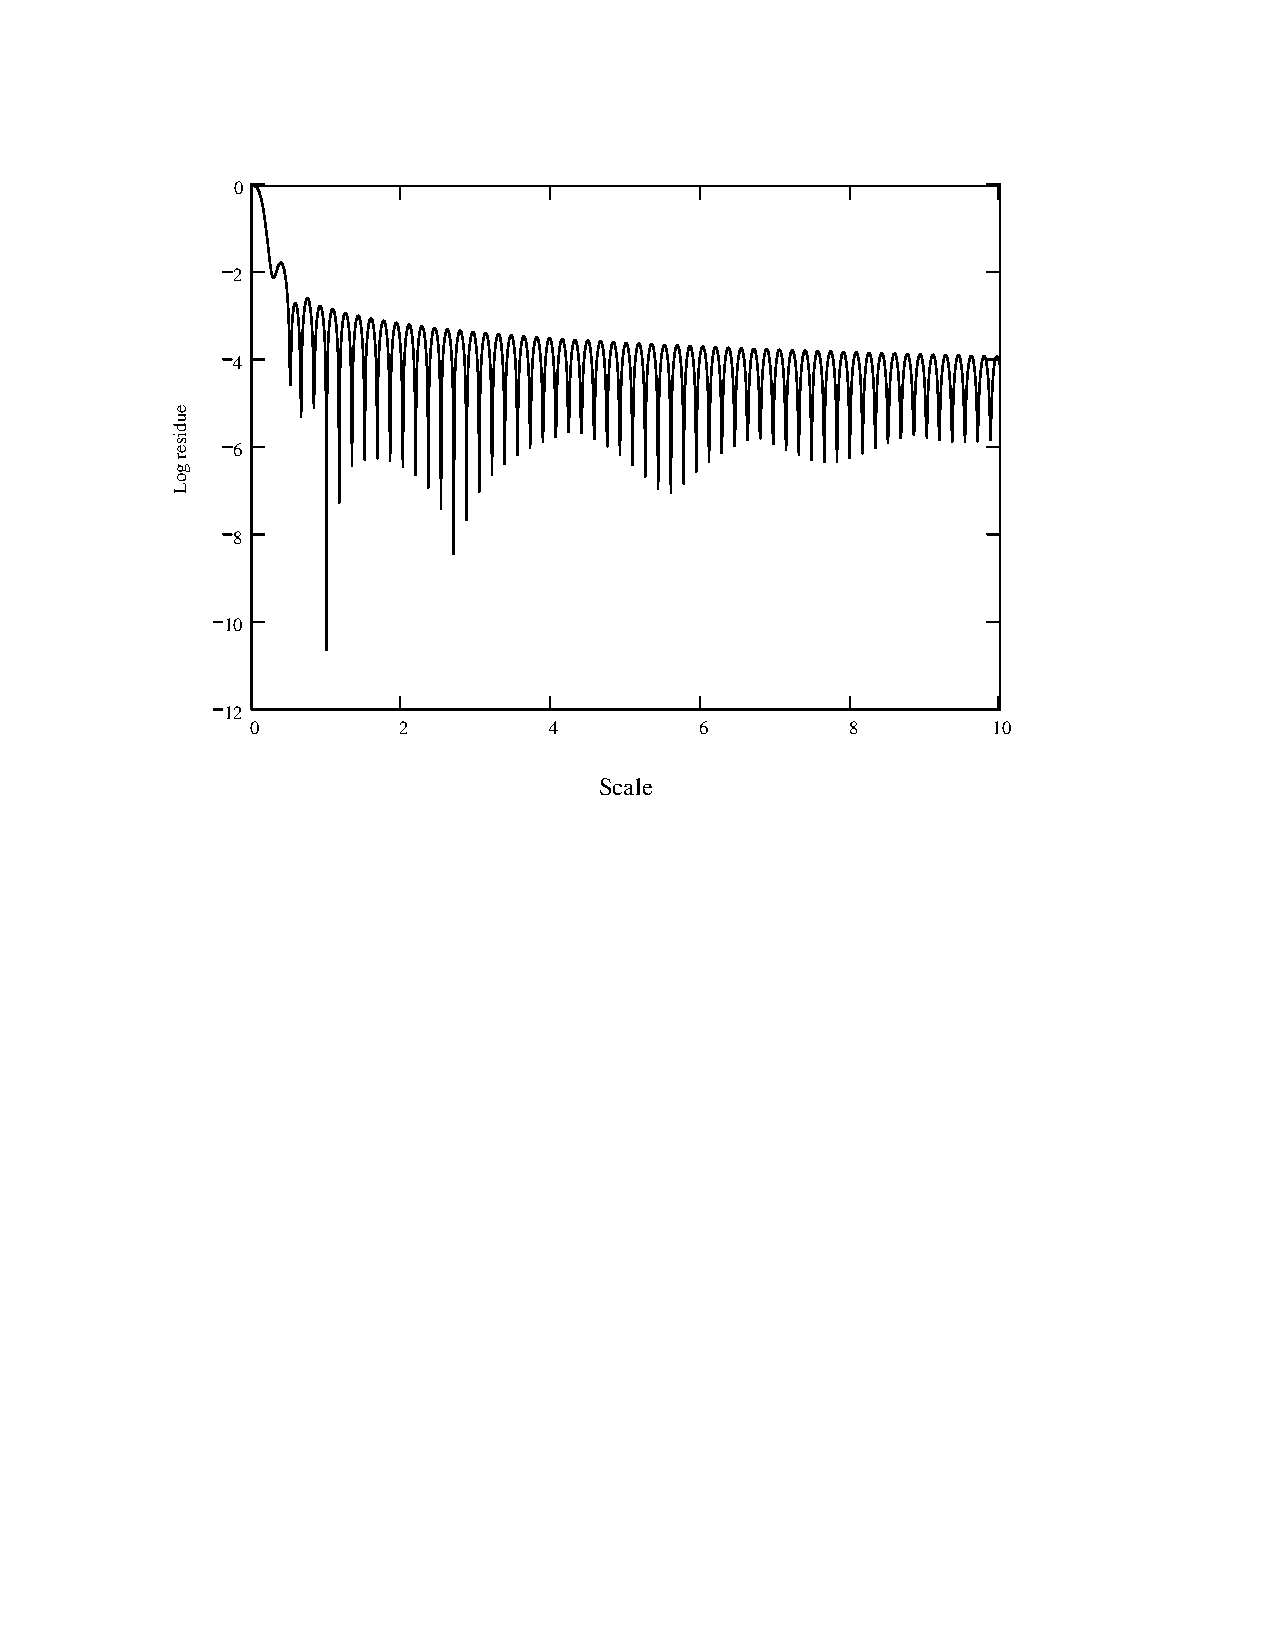
\includegraphics[bb=30 415 489 715]
{scale_two-color/scale_two-color.pdf}
}
\caption[Amplitude ``robustness'' of the two color STIRAP]{Amplitude ``robustness'' of the two color STIRAP. The optimal solution in Figure \ref{solution 2 pulses} is allowed to vary in pulse height by the ``scale'' factor (both pulses are scaled simultaneously) and the resulting residue, as defined by Equation \ref{phi prime} is plotted as a function of the scale. The narrow downward ``spikes'' are real; however, their depth may not be acurately displayed here due to ``aliasing'' effects between the regular spacing of computer generated points and the sharp spikes. In short, the residue is around $10^{-3}$ for most of the range of the ``scale'' factor, except for numerous ``pits'' where the residue drops to $10^{-6}$ or less.}
\label{scale_two-color}
\end{figure}
%----------------------------------------------------------------------------
